\section{Introduction}
Camera Networks (CN) are increasingly popular in various domains, such as 
smart cities, smart manufacturing, and smart agriculture, to name a few. 
All cameras must be carefully calibrated to collect the desired information 
with the required quality. 
The collective coverage of the CN directly affects the achievable information 
quality concerning accuracy and completeness. In particular, the intrinsic 
and extrinsic configuration of the cameras decides on the achievable 
information quality.

Intrinsic Calibration finds a camera's intrinsic parameters, such as its 
focal length, principal point, or distortion coefficients. They describe 
the internal properties of the camera. Extrinsic Calibration, on the other 
hand, uncovers the camera's pose, describing its position and orientation in 
a shared world coordinate system.

In this work, we focus on the extrinsic configuration of a CN. Calibrating 
large CNs is challenging as it quickly becomes time and 
cost-intensive when the CN's size grows. Although many methods exist for 
extrinsic camera calibration, they often prove impractical in large-scale, 
real-world scenarios.

% Feature: Converage
Understanding the coverage of the CN is crucial for identifying 
potential blind spots. However, relying solely on a camera's field of view 
may not provide an accurate representation. Despite a camera's lens 
suggesting a wide field of view, trees or other structures 
can obscure crucial elements within the scene. To address this, we 
propose defining the camera's actual captured portion of the scene as 
its effective field of view.

\begin{figure}
	\centering
	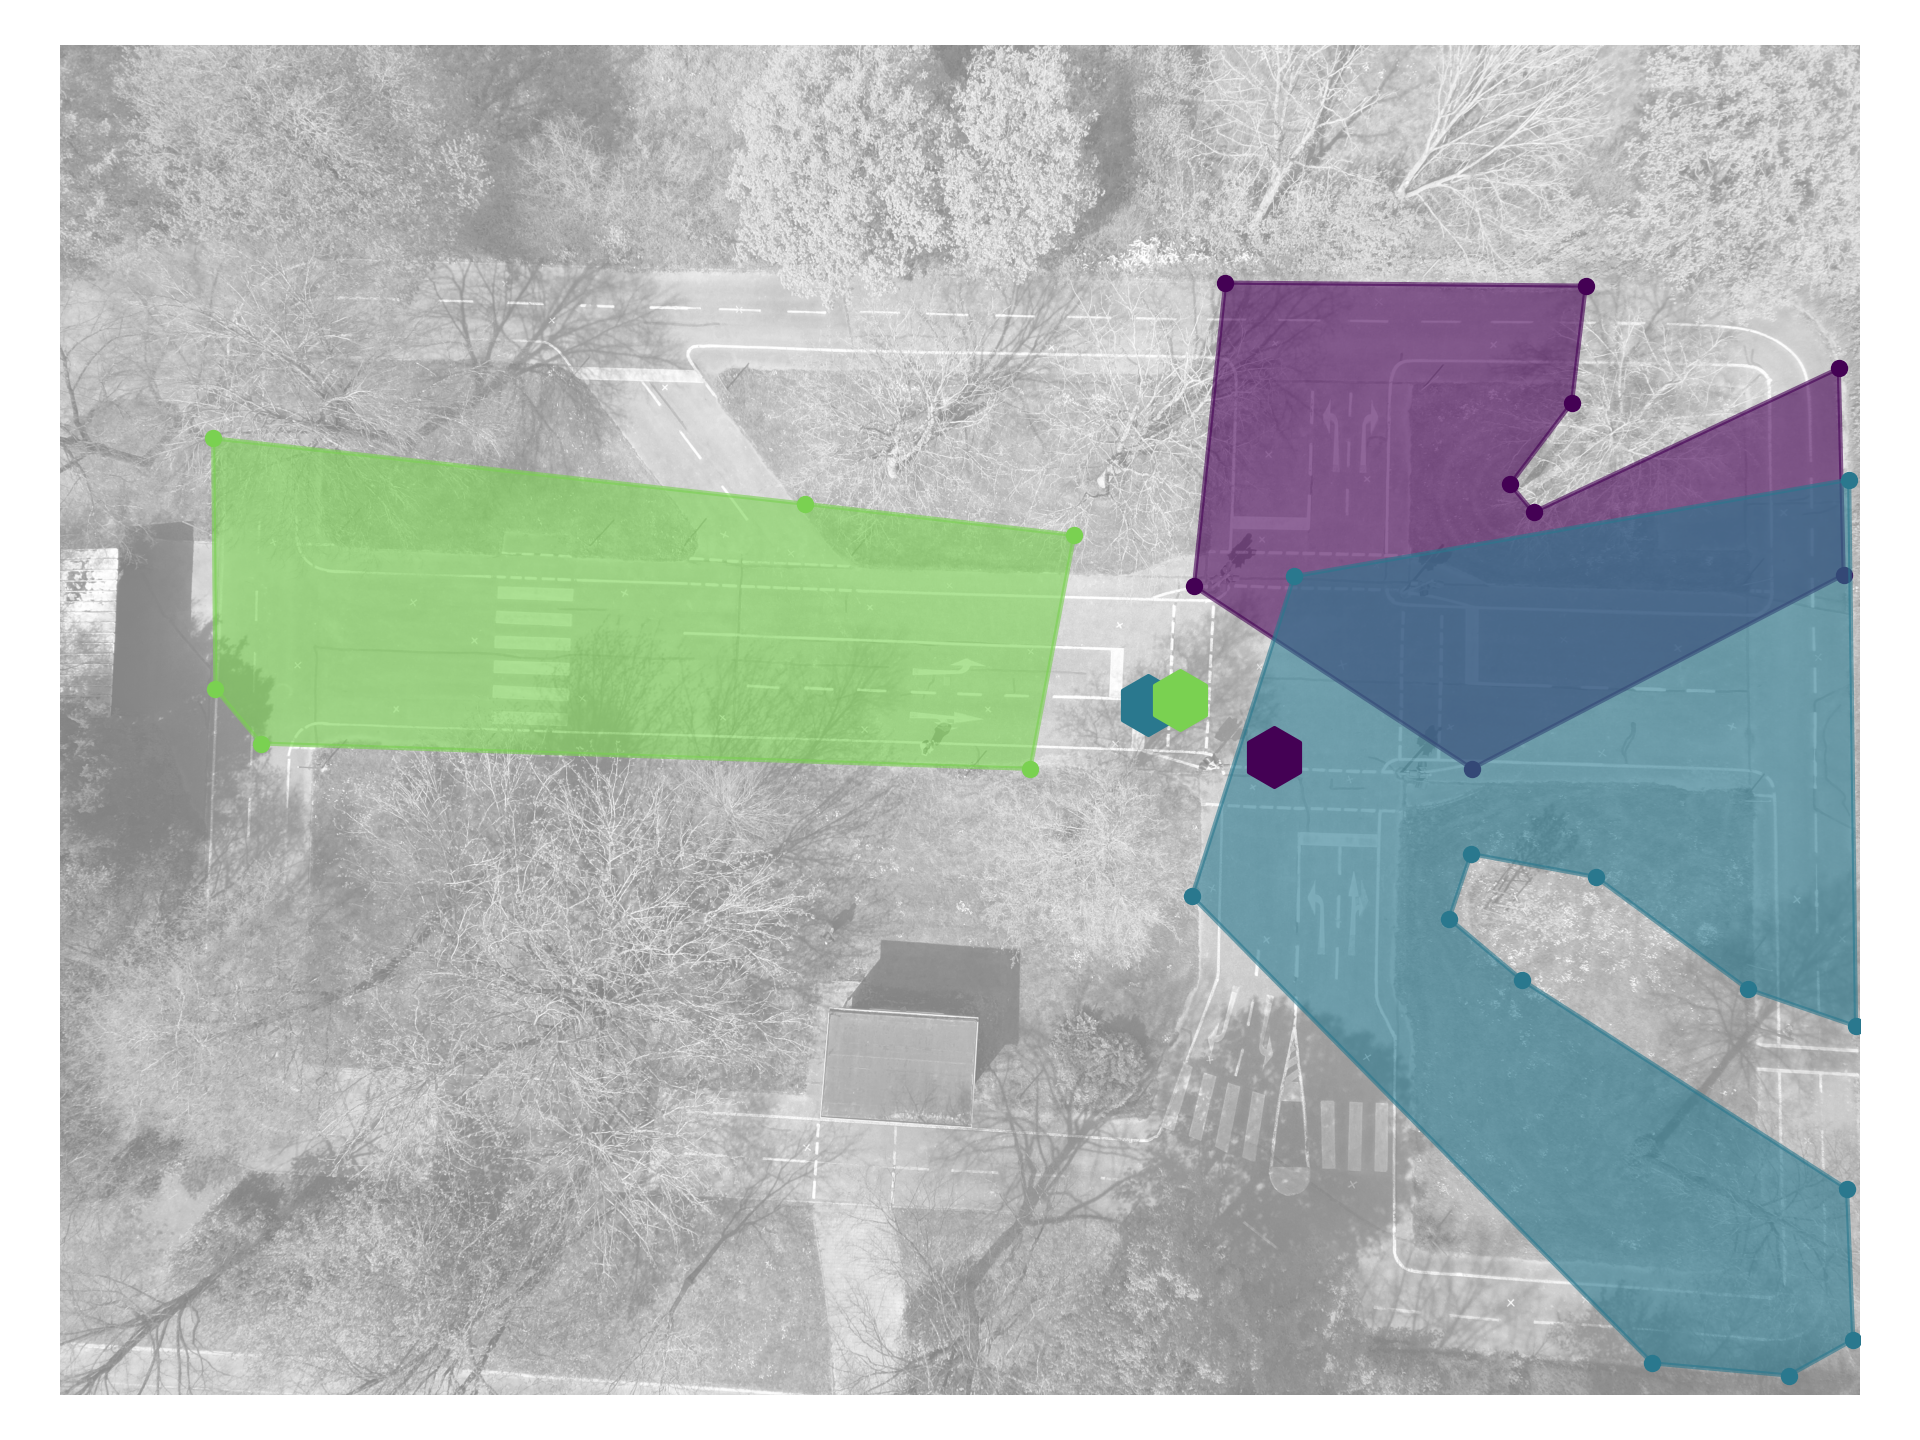
\includegraphics[width=0.4\textwidth]{figures/overview.png}
	\caption{
	The location of three cameras (hexagon) and their effective
	field of view. 
	}
	\label{fig:overview}
\end{figure}

% Eingrenzung
This work focuses on mono-modal approaches using images from statically 
mounted cameras. Compared to lidar sensors, cameras are relatively low-cost 
and provide more details for classification tasks. However, images lose 
depth information. 

% Addon: Homography accuracy
Our method uses homographies, which per se assume planar scenes. However, 
this assumption is violated within real-world conditions. 
Therefore, we provide an exhaustive investigation of 
homographies in real-world conditions and examine relevant influencing factors. 
Accordingly, we derive best practices for using homographies in real-world 
scenes.

The key contributions of this paper are:
\begin{enumerate}
	\item ESCal, a method that semi-automatically determines extrinsic parameters for 
		each camera within an arbitrary CN\textemdash without requiring overlapping fields of view.
	\item A technique for measuring, evaluating, and adjusting a CN's effective 
		coverage.
	\item We present a set of countermeasures to determine homographies 
		accurately and robustly within real-world settings. 
	\item We demonstrate through intensive experiments that the proposed method 
		is easy to use, fast, scalable, and sufficiently accurate for most 
		CN use cases.
\end{enumerate}

The remainder of this paper is structured as follows.
Section \ref{sec:related_work} reviews the state of the art and compares 
our approach to related literature. Section \ref{sec:background} provides 
the necessary preliminaries and notation. Section \ref{sec:problem} details 
the problem statement. Section \ref{sec:solution} describes ESCal, our proposed 
solution. In Section \ref{sec:experiments}, we present our experiments and 
their results. Finally, Section \ref{sec:conclusion} concludes the paper.
